% 3_methodology.tex

\cleardoublepage
\chapter{Launch Vehicle Design and Simulation}\label{chapter:methodology}


\textcolor{red}{First stage has been changed to 8.5m , with 1m of space for connection, also 70\% thrust. Will include a section describing the launch site (ELA). Will put in pictures defining sun synch orbit, and more detail about sun synchronous orbit}

\textcolor{red}{Fuel tanks are depleted cylindrical first, to move CG for stability, and to minimise slosh (maybe point towards concorde here)}

In order to be competitive in the emerging small satellite market, a small satellite launcher must be cost-effective, reliable, and capable of launching on a flexible schedule. The inclusion of airbreathing engines within a small satellite launch system has the potential for improving cost effectiveness compared to disposable rocket-powered launchers, by allowing partial reusability of a launch system. The airbreathing engine most appropriate for small satellite launch systems are scramjet engines, which operate efficiently within the hypersonic regime, with the capability to operate over a relatively large Mach number range compared to turbojet or ramjet engines. A launch system incorporating scramjets must necessarily include two rocket-powered flight stages; a first stage rocket to accelerate the system from launch to the minimum operational Mach number of the ramjet or scramjet engines; and a third stage rocket to accelerate the payload at exoatmospheric conditions and place it into the correct orbit. 
This chapter presents the design and modelling of a rocket-scramjet-rocket launch system in which the scramjet stage is reusable for multiple launches. 
For this launch system to be economically viable, the scramjet stage must be capable of accelerating to a high Mach number, and then returning to its initial launch site for re-use. Returning to the initial launch site removes the need for costly and time-consuming transportation, and allows the refurbishment and refuelling of the scramjet stage to begin immediately. 
This rocket-scramjet-rocket launch system is designed to launch satellites on the order of 200kg to a 567km altitude sun-synchronous orbit. A sun synchronous orbit is targeted as it is a potentially desirable orbit for small satellite missions, being advantageous for imaging purposes due to its low altitude and consistently timed overpasses. This orbit is consistent with previous studies which have investigated rocket-scramjet-rocket small satellite launch systems, allowing the missions developed in this study to be compared and contrasted to unoptimised mission profiles. 
The rocket-scramjet-rocket launch system described in this chapter is used as a representative model for an airbreathing, partially-reusable, multi-stage small satellite launcher. 



\begin{figure}[ht]
	\centering
	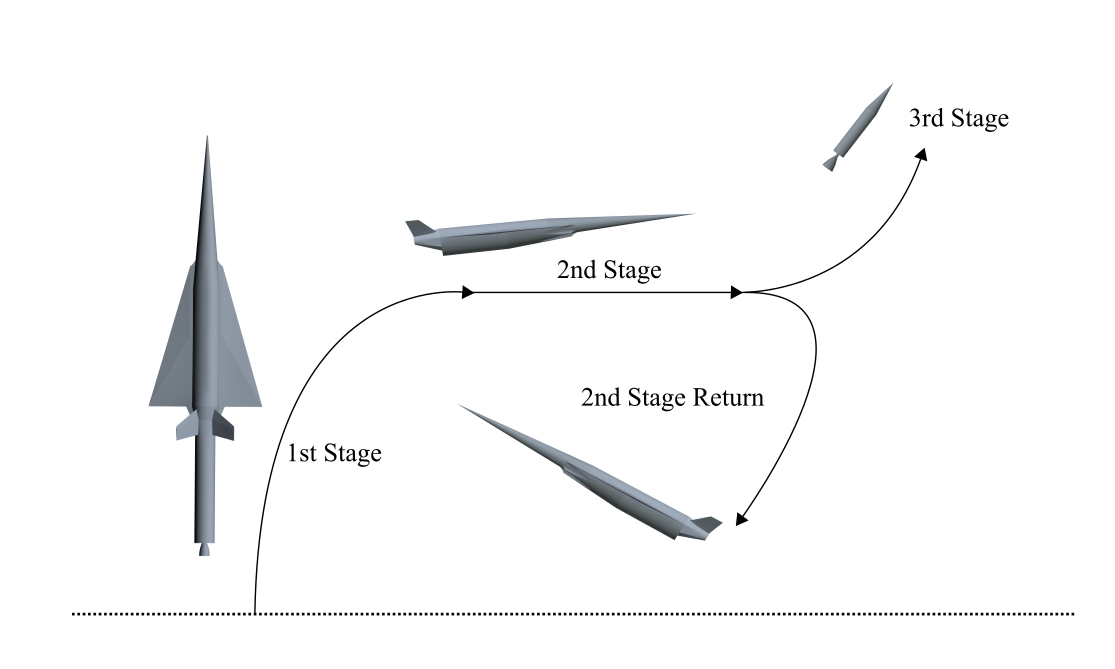
\includegraphics[width=0.9\linewidth]{figures/3_vehicle_design/Trajsimple}
	\caption{The launch process of the rocket-scramjet-rocket launch system, presented in simplified form.}
	\label{fig:Trajsimple}
\end{figure}

 The rocket-scramjet-rocket launch system used in this study has been designed based on the SPARTAN scramjet accelerator developed by Preller \& Smart [CITATIONXX]. The SPARTAN is a scramjet-powered accelerator being developed by The University of Queensland and Hypersonix. The SPARTAN has been designed for small satellite launches, as part of a rocket-scramjet-rocket launch system.
 The SPARTAN has been used as the basis for design of the launch system, as it is the most complex stage of the system, and its unique trajectory requirements drive the design of the other stages.
 The trajectory of a launch system involving scramjet propulsion is significantly different to that of a fully rocket-powered launch system. Figure \ref{fig:Trajsimple} shows a simplified representation of the launch trajectory for the vehicle simulated in this study. The operation of the scramjet engine requires in-atmosphere flight, at high dynamic pressure conditions for long periods of time. The launch system must be designed to withstand the high structural loading and heating generated by flight at these conditions. 
 The SPARTAN vehicle is mounted to the front of the first stage rocket. The launch system is launched vertically under rocket power, from a traditional small rocket launch facility. 
 This configuration allows the SPARTAN to take the brunt of the aerodynamic forces and heating, as well as allowing the use of the control surfaces of the SPARTAN. During first stage rocket operation, the launch system pitches rapidly, reaching close to horizontal flight to allow the SPARTAN to stay at high dynamic pressure conditions. The SPARTAN is accelerated to its minimum operating velocity of approximately Mach 5, at which point separation occurs. The SPARTAN's four scramjet engines are ignited, and The SPARTAN is accelerated through the atmosphere, reaching approximately Mach 9. At this point, the specific impulse of the scramjet engines, and thus the efficiency of the SPARTAN, have decreased, and the third stage rocket is separated. The third stage rocket accelerates and performs a pull-up, before cutting its engine and coasting out of the atmosphere. Once the rocket is exoatmospheric, the engine is reignited, performing first a circularisation burn, and then a Hohmann transfer to the intended orbit. Meanwhile, the SPARTAN banks and executes a fly-back manoeuvre to return to its initial launch site. The SPARTAN extends landing gear, and lands on a traditional runway in the style of a conventional aircraft. The SPARTAN is able to be rapidly refurbished and remounted for further launches. To fulfil the requirements of this trajectory, The SPARTAN must be able to fly and manoeuvre at all Mach numbers from 0 to 9, as well as being able to withstand high structural and heating loads without significant deterioration.
 
 The three stage launch system incorporating the SPARTAN is shown in Figures \ref{fig:NoInternal} \& \ref{fig:INTERNALS}. 
 The size and external design of the SPARTAN scramjet accelerator are used exactly as defined for the Baseline SPARTAN vehicle defined by Preller \& Smart. The internal layout has been designed for the SPARTAN to carry a large fuel volume while allowing the third stage to fit within the fuselage. 
 The first and third stages have been designed for this study. The third stage rocket replaces the third stage used in previous SPARTAN studies, which was powered by a Pratt \& Whitney RL-10-3A engine, with a rocket stage powered by a SpaceX Kestrel engine.  
The SPARTAN design is presented first, as the design of the SPARTAN drives the design of the first and third stage rockets. 


\begin{figure}[ht]
	\centering
	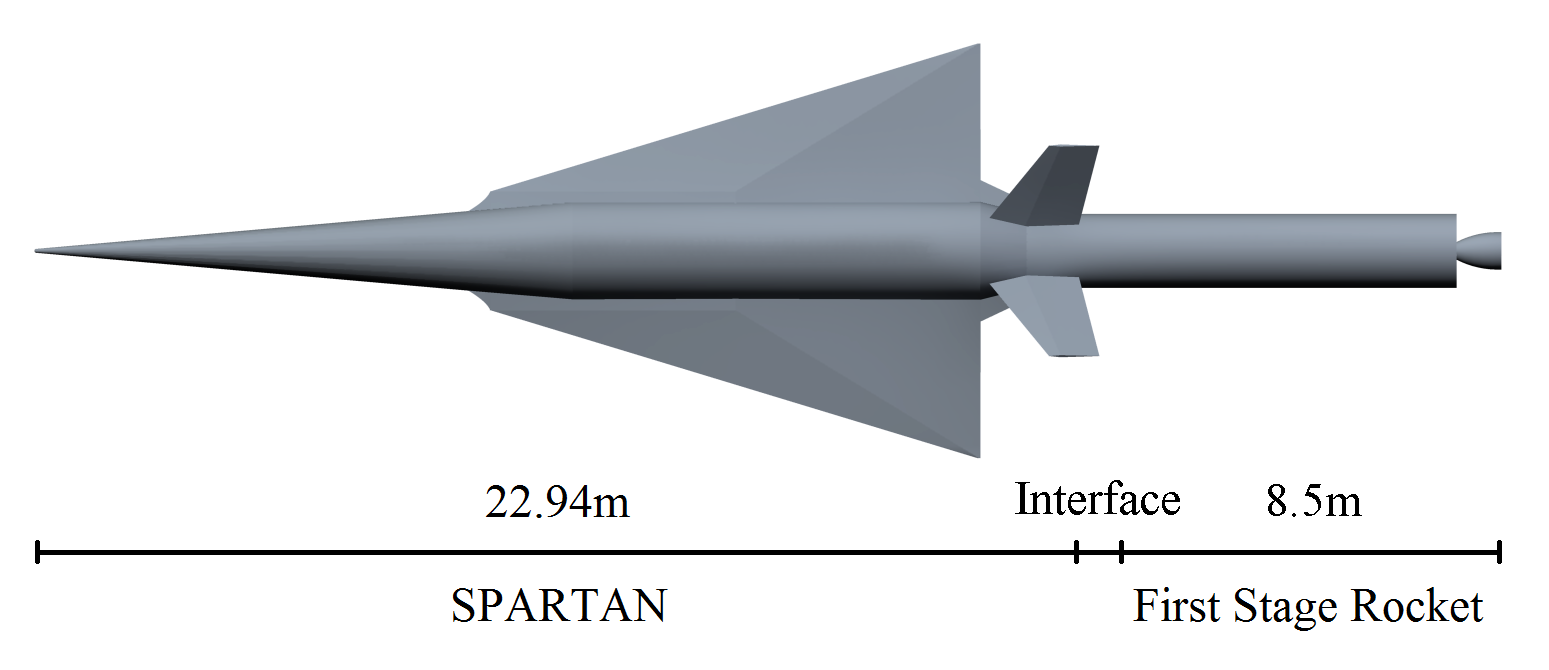
\includegraphics[width=0.7\linewidth]{figures/3_vehicle_design/NoInternal}
	\caption{The rocket-scramjet-rocket launch system, top view, showing the SPARTAN and first stage.}
	\label{fig:NoInternal}
\end{figure}

\begin{figure}[ht]
	\centering
	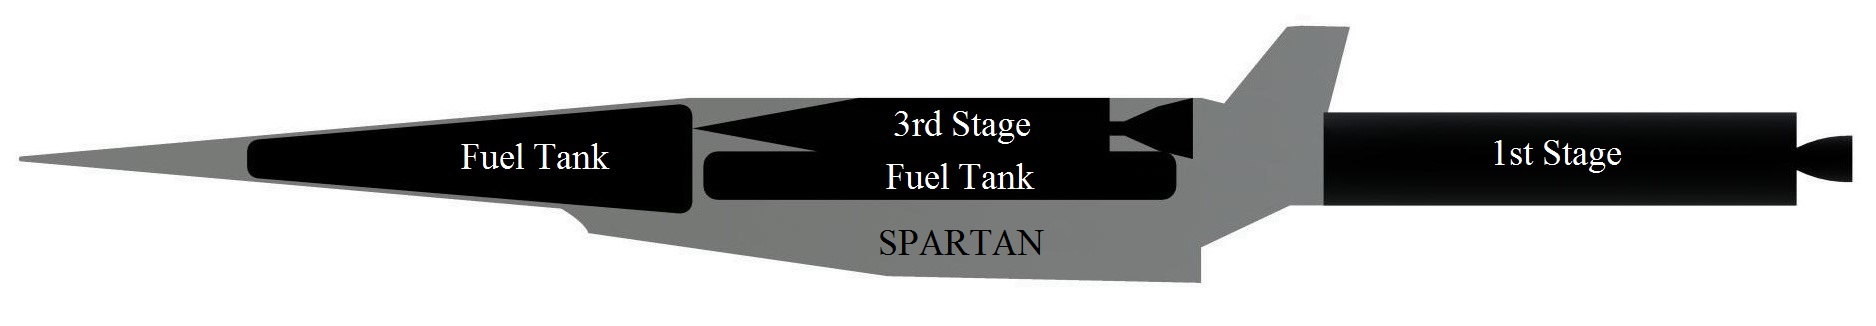
\includegraphics[width=0.7\linewidth]{figures/3_vehicle_design/INTERNALS}
	\caption{The rocket-scramjet-rocket launch system, side view, showing the SPARTAN and fuel tanks, along with the third and first stages.}
	\label{fig:INTERNALS}
\end{figure}









	
	
	\section{Second Stage Scramjet}

	
		\subsection{The SPARTAN Accelerator}
		
		The SPARTAN vehicle in this study is designed based on the work by Preller \& Smart CITATION. The SPARTAN is 22.94m long, with a frontal cone half angle of 5$^\circ$ [CITEXX DAWIDS THESIS]. A mass breakdown of the SPARTAN is shown in Table \ref{tab:MassBreakdown}, adapted from [CITAXX Dawids thesis]. The fuel tank sizes and total fuel mass are sized to accommodate for the Kestrel-powered third stage, described in Section \ref{sec:ThirdStageBaseline}.
		\begin{table}[h]
		\begin{tabular}{|c|c|c|c|c|c|c|c|}
			\hline  \textbf{Part} & Fuselage & Wings & Tanks & Systems & Landing Gear & Scramjets & Fuel \\ 
			\hline \textbf{Mass} (kg) & 2861.6 & 350.7 & 179.4 & 707.5 & 188.9 & 669.0 & 1562.0 \\ 
			\hline 
		\end{tabular} 
		\caption{Mass breakdown of the modified SPARTAN vehicle.}
		\label{tab:MassBreakdown}
		\end{table}
This study assumes that the third stage is stored within the fuselage of the SPARTAN for simplicity. It is assumed that the release mechanism for the third stage is able to be situated within the available space surrounding the third stage, however the release mechanism is not considered further in this study. 
		
		
		% LH2 density
		 %http://webbook.nist.gov/cgi/fluid.cgi?Action=Load&ID=C1333740&Type=SatT&Digits=5&PLow=.5&PHigh=1.5&PInc=.1&RefState=DEF&TUnit=K&PUnit=atm&DUnit=kg/m3&HUnit=kJ/mol&WUnit=m/s&VisUnit=uPa*s&STUnit=N/m%

		The fuel tanks are sized to fit around the kestrel-powered third stage. There are three fuel tanks; two cylindrical tanks situated underneath the third stage; and a truncated conical tank in the nose. The conical fuel tank is designed to fit immediately forward of the third stage. This fuel tank is 8m long, leaving 1.47m$^3$ of space in the nose for cooling systems, frontal landing gear and any additional systems or sensors which are necessary in the nose cone. The cylindrical tanks are positioned underneath and slightly to either side of the third stage, leaving space underneath for vehicle systems. The cylindrical fuel tanks are designed to be 8.5m long, with diameters of 0.87m, sized to give a nominal total tank volume of 22m$^3$.
The fuel tanks hold a total of 1562kg of LH2 fuel. This assumes an LH2 density of 71kg/m3, slightly denser than LH2 at phase transition point at 1 atm.
The mass of the fuel tanks is scaled from Dawid Preller's Baseline vehicle model of the SPARTAN, giving a total fuel tank mass of 179.4kg.
		
		


\subsection{Propulsion}


The SPARTAN is powered by four underslung scramjet engines, fuelled by liquid hydrogen. These engines are Rectangular To Elliptical Shape Transition (REST) engines, configured to allow for a conical forebody (C-REST). REST engines have a rectangular to elliptical shape transition inlet, and an elliptical combustor, offering simplicity in design as well as reduced thermal loading and viscous drag compared to scramjets with planar geometries \cite{Suraweera2009}.  REST engines are also specifically designed to operate over a wide range of Mach numbers, and at off design conditions, making them particularly applicable to use on scramjet accelerator vehicles. 


\subsubsection{Propulsion Modelling}\label{sec:Propulsion}

The properties of the C-REST scramjet engines must be modelled at every flight condition which the SPARTAN may experience during its flight. The thrust generated by the C-REST engines determines how rapidly the SPARTAN accelerates, and the efficiency of the engines determines the total flight time, and influences the separation point of the third stage rocket. The C-REST engines are simulated separately to the aerodynamic simulations of the SPARTAN, using quasi-1D simulation for simplicity. The engine model takes the conditions at the inlet, and calculates the exit conditions and propulsive properties of the engine. The engine exit conditions are added into the aerodynamic simulations and the propulsive properties are used in the simulated vehicle model.

Before the flow enters the engine, it is affected by the conical shock generated by the forebody of the SPARTAN.
Figure \ref{fig:SPARTANEngineshock} shows the locations of the flow properties which are necessary to calculate engine performance. The ambient atmospheric conditions are calculated by interpolation using the 1976 NASA Atmospheric properties\cite{Administration1976}.
The flow properties at the inlet of the engines is calculated using the Tayor-Maccoll analysis method for conical shocks[CitationXX]. This calculation is performed in the cone\_shoot program provided for this study by Prof. Michael Smart[CitationXX?]. The flow conditions following the conical shock are shown in Figure \ref{fig:ConicalShock}.  

\begin{figure}[ht]
\centering
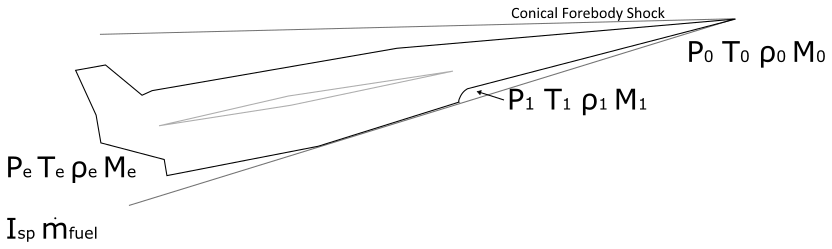
\includegraphics[width=0.7\linewidth]{figures/3_vehicle_design/SPARTANEngineshock}
\caption{The locations of conditions relevant to C-REST engine simulation. }
\label{fig:SPARTANEngineshock}
\end{figure}


\begin{figure}
\begin{subfigure}{.5\textwidth}
\centering
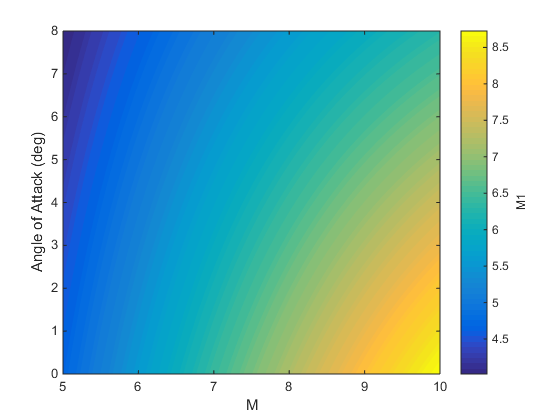
\includegraphics[width=0.99\linewidth]{figures/3_vehicle_design/ConicalM}
\caption{Mach number.}
\label{fig:ConicalM}
\end{subfigure}
\begin{subfigure}{.5\textwidth}
\centering
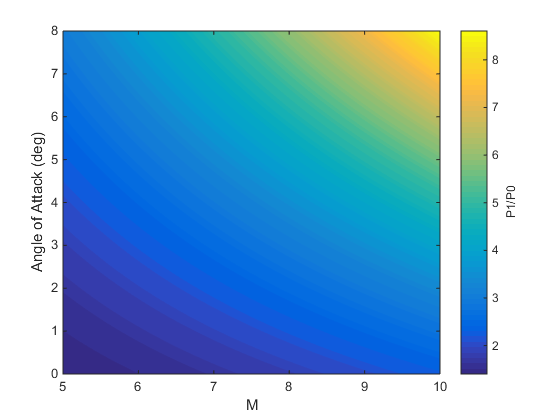
\includegraphics[width=0.99\linewidth]{figures/3_vehicle_design/ConicalP}
\caption{Pressure ratio.}
\label{fig:ConicalP}
\end{subfigure}
\begin{subfigure}{.5\textwidth}
\centering
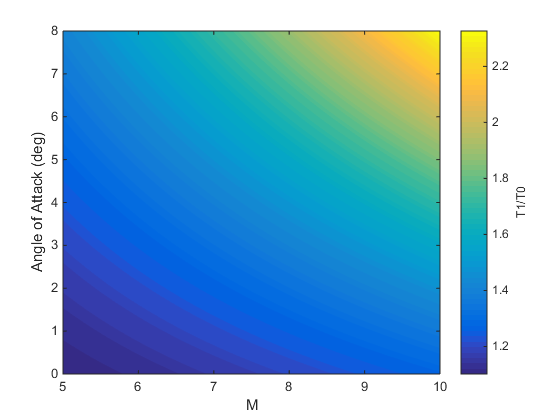
\includegraphics[width=0.99\linewidth]{figures/3_vehicle_design/ConicalT}
\caption{Temperature ratio.}
\label{fig:ConicalT}
\end{subfigure}
\caption{Flow conditions after the conical shock generated by the vehicle nose cone. Figure a) shows the Mach number, b) shows the pressure ratio, and c) shows the temperature ratio following the conical shock.}
\label{fig:ConicalShock}
\end{figure}

 The engine model used is a CRESTM10 database\cite{Preller2017,Preller2018}, analysed using quasi-1D simulation and provided for this study by Prof. Michael Smart. This database has previously been used in simulations of the SPARTAN, as explained in Section \ref{sec:enginemodel}.
This database provides data points of engine performance over inlet conditions within the operational range, at 50kPa dynamic pressure equivalent conditions. The specific impulse data set is shown in Figure \ref{fig:ISPinterp}. This data is interpolated using bivariate splines for the given inlet conditions, to calculate specific impulse produced by the engine. During flight the C-REST inlet conditions will stay within the region bounded by the available data. However, for the purposes of the trajectory optimisation, it is necessary for the vehicle model to be able to extrapolate for ISP and equivalence ratio data. This extrapolation is linear, and is used to drive the optimisation, but does not directly affect the final solution. 
For operation at high Mach numbers, the fuel mass flow rate is assumed to be stoichiometric, so that $\dot{m_f}$ = $0.0291\dot{m}$. This ensures that the scramjet engines are performing at high efficiency throughout the acceleration of the scramjet stage. 
\begin{figure}[ht]
	\centering
	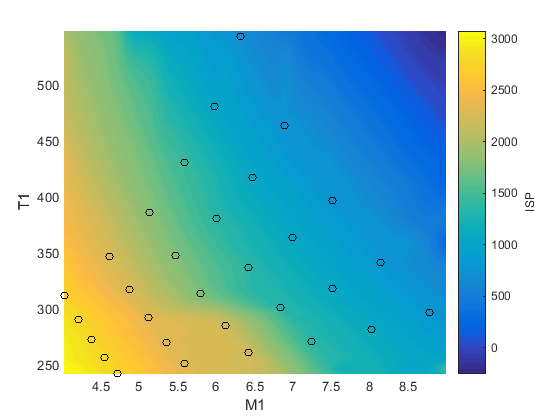
\includegraphics[width=0.6\linewidth]{figures/3_vehicle_design/ISPinterp}
	\caption{Specific impulse of the CRESTM10 engines with input temperature and Mach number. Available data points are indicated.}
	\label{fig:ISPinterp}
\end{figure}
However, the C-REST engine is a fixed geometry engine, primarily designed for operability at high Mach numbers\cite{Preller2017}. At lower Mach numbers, the addition of excessive fuel may cause the engine to choke and unstart, resulting in total loss of thrust\cite{Preller2017}. To avoid unstart, an equivalence ratio ($\phi$) of less than 1 is set at low Mach numbers. The equivalence ratio interpolation is linear, as the number of data points available for interpolation is low. The equivalence ratio over the range of SPARTAN operation is shown in Figure \ref{fig:EquivalenceRatioInterp}.
\begin{figure}[ht]
	\centering
	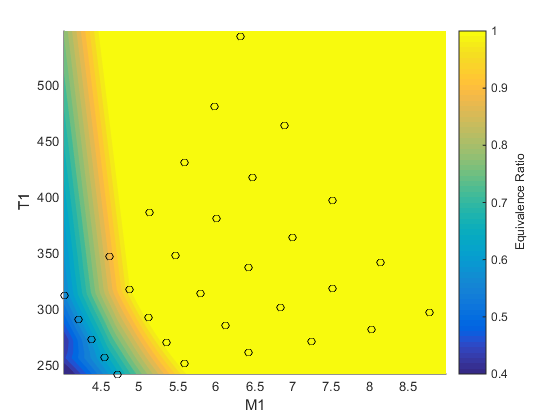
\includegraphics[width=0.6\linewidth]{figures/3_vehicle_design/EquivalenceRatioInterp}
	\caption{Operable equivalence ratio of the CRESTM10 engines with input temperature and Mach number. Available data points are indicated.}
	\label{fig:EquivalenceRatioInterp}
\end{figure}
The fuel mass flow rate is determined by approximating the flow into the inlet as an ideal gas; 

$\dot{m} = 0.9 m_c A_{cap} P_0 M_0 \sqrt{\dfrac{\gamma_0}{R_{air} T_0}}$,

$\dot{m}_{fuel} = (\dfrac{m_{fuel}}{m_{ox}} )_{st} \phi \dot{m}$

The multiplier of 0.9 is an approximate term included to account for losses due to asymmetry within the engine\cite{Preller2018}. 
The thrust for each engine, $T$, is obtained by inclusion of the interpolated specific impulse, ie. 

$T = g_0\dot{m}I_{sp}$. 







		
		
		\subsection{The Aerodynamics of the SPARTAN}\label{sec:aero}
		
		\textit{Note: Viscous correction will be added to the aerodynamic database, calculated by Alexander Ward. The additional thrust obtained by the nozzle exit and boat tail is currently being computed in Cart3d and will be added to the propulsive database.}
		
		
In order for the trajectory of the SPARTAN to be successfully simulated and optimised, the aerodynamics of the SPARTAN must be calculated for the large range of flight conditions experienced during the acceleration and return flights. 
The aerodynamics of the SPARTAN are calculated at set flight conditions covering the breadth of necessary conditions, and the results are tabulated in databases. During simulation, the aerodynamics of the SPARTAN are determined by interpolation over the aerodynamic databases using bivariate splines. 


The aerodynamics are calculated for Mach numbers between 0-10, angles of attack between 0$^\circ$ and 10$^\circ$, and for altitudes between 0-40km. Separate aerodynamic simulations are performed for engine-on and engine-off conditions, as the operation of the scramjet engines changes the aerodynamic characteristics of the SPARTAN significantly. When the engines are powered on, the engines are generating thrust on the internal nozzle, as well as on the boat-tail and base.  When the scramjet engines are not operational air flows through the flowpath without fuel injection, generating a large amount of drag. 
The drag, lift and moment coefficients are determined by interpolating for Mach number, angle of attack, altitude, and centre of gravity as it shifts during flight.
		The drag and lift produced by each stage of the vehicle are calculated using the standard definition of the aerodynamic coefficients:
		
		\begin{equation}
		F_d = \frac{1}{2}\rho c_d v^2 A ,
		\end{equation}
		
		\begin{equation}
		F_L = \frac{1}{2}\rho c_L v^2 A .
		\end{equation}
		
		\subsubsection{CART3D}

				The aerodynamics of the SPARTAN have been calculated using CART3D, an inviscid CFD package used in the preliminary design of aerospace vehicles. Cart3D utilises adjoint mesh adaption with a Cartesian cut-cells approach to produce an iteratively refined mesh to fit a flow solution. CART3D is
				been used to generate the aerodynamic database of the SPARTAN vehicle due to its applicability in both the subsonic
				and supersonic regimes, and its robustness across multiple flow solutions [16]. CART3D has previously been used to
				analyse hypersonic vehicles, and has shown fair agreement with experimental data across multiple studies CITATIONXX.
				
						The CART3D Meshes are initiated with an outer boundary distance of 40 times the vehicle length. This boundary distance was observed to produce suitable free stream conditions and good mesh convergence. Nine mesh adaption levels are used. Nine levels have been observed to generally produce good convergence, with moderate computation times of 1-3 hours per simulation. The convergence of the residuals and forces are investigated to ascertain if a solution has converged. Figure XX shows an example solution validation for Mach 7, 2$^\circ$ angle of attack, engine-on conditions. Good convergence can be observed in the force functionals, with a corresponding decrease in the residual values indicating solution convergence.  
						
						
						\textit{A CART3D validation image will be inserted here, showing decreasing residuals and converging functionals.}
		
		
		\subsubsection{Trim Analysis}\label{sec:trim}
		
		The SPARTAN is trimmed during flight using control surfaces on the wings. The trim is incorporated into the aerodynamic databases prior to trajectory simulation, assuming that the SPARTAN is trimmed at all conditions during flight. 		
		\begin{figure}[ht]
			\centering
			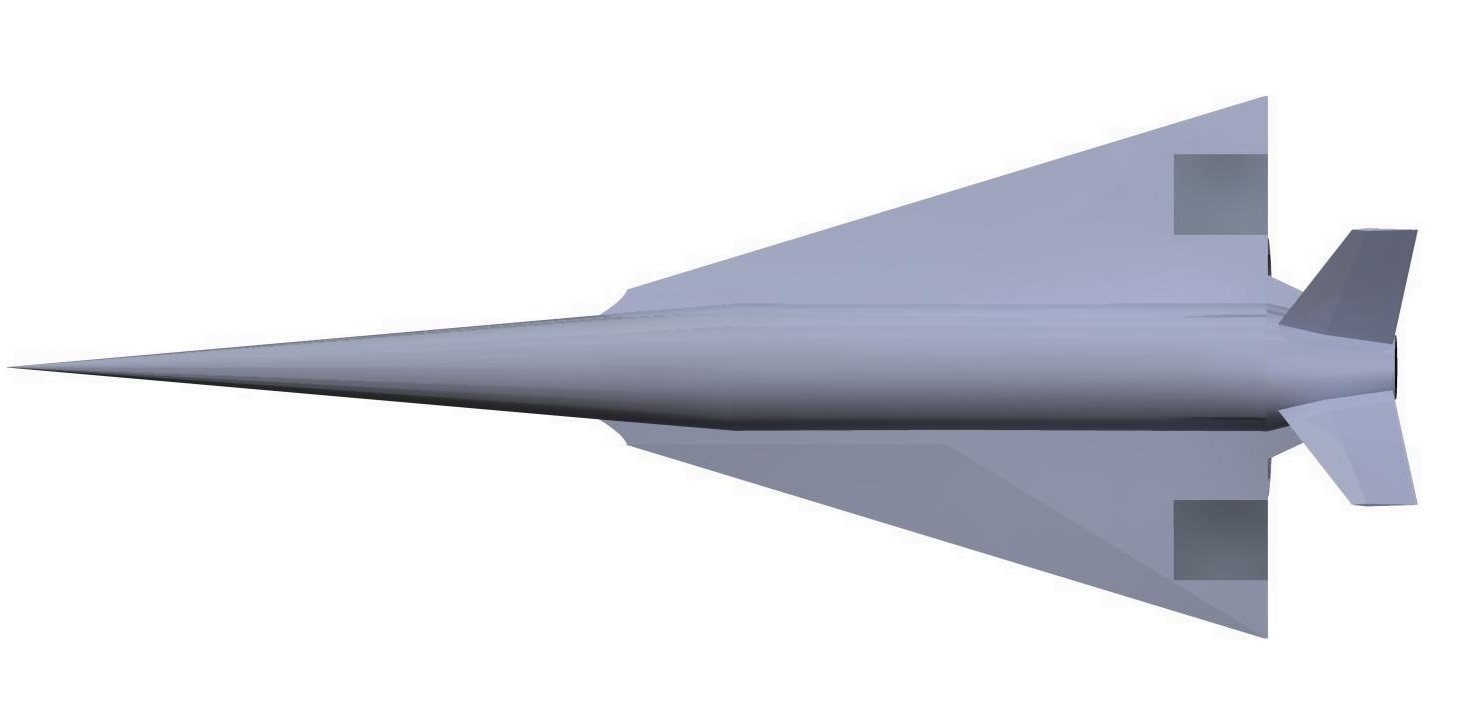
\includegraphics[width=0.6\linewidth]{figures/3_vehicle_design/SPARTAN_FLAPS}
			\caption{SPARTAN model showing control surfaces. \textit{Dimensions will be included.}}
			\label{fig:SPARTAN_FLAPS}
		\end{figure}
		The SPARTAN is trimmed using control surfaces on the wings, shown in figure \ref{fig:SPARTAN_FLAPS}. 
		Trim is determined by calculating the aerodynamic moment coefficient with zero flap deflection, then calculating the flap deflection necessary to balance the aerodynamic moments to zero. The moment generated by the body and wings of the SPARTAN is balanced by the moment generated by the ailerons, as well as the thrust moments on the engines and boat tail, when the C-REST engines are powered on. The force balance on the SPARTAN is shown in Figure \ref{fig:SPARTANForces}. This trim balancing is calculated prior to trajectory optimisation for computational efficiency.
		\begin{figure}[ht]
			\centering
			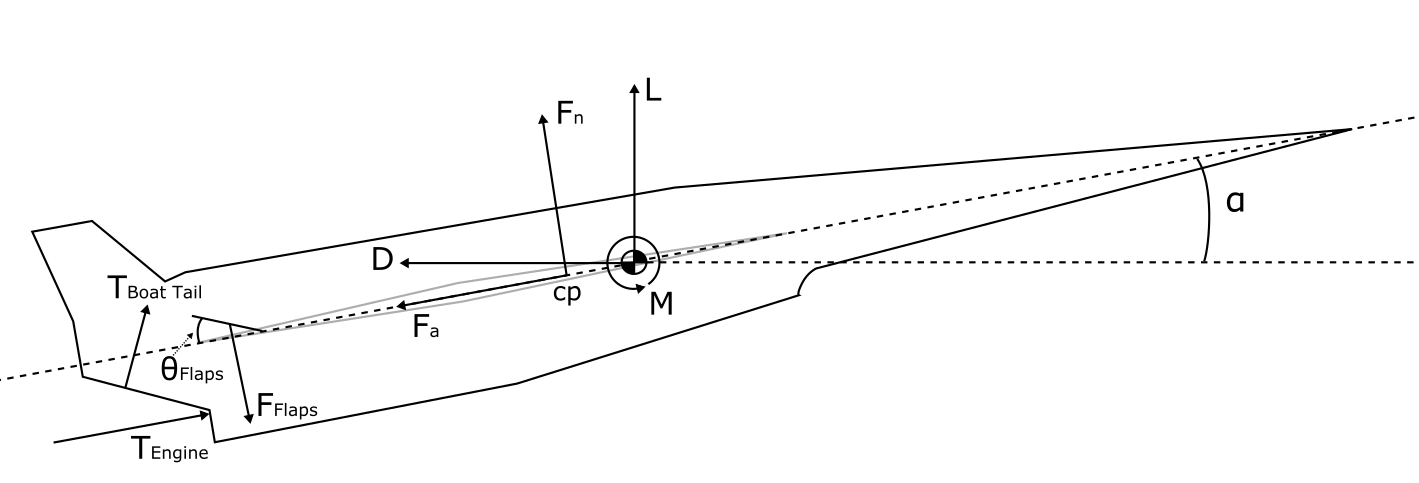
\includegraphics[width=0.7\linewidth]{figures/3_vehicle_design/SPARTANForces}
			\caption{The forces on the SPARTAN during flight.}
			\label{fig:SPARTANForces}
		\end{figure}
		
		The centre of gravity of the SPARTAN is calculated using CREO. The centre of gravity varies during flight due to fuel consumption and third stage release, changing the necessary flap deflections for trim. Consequently, aerodynamic databases are created for centre of gravity conditions of; 
		\begin{itemize}
			\item full fuel including third stage,
			\item empty of fuel including third stage,
			\item empty of fuel after third stage release.
		\end{itemize}
		At each of these conditions, aerodynamic coefficients and flap deflections necessary for trim are calculated.  For simplicity, it is assumed that structural, systems and landing gear masses are homogeneously distributed throughout the centre fuselage of the SPARTAN. The calculated centre of gravity for the SPARTAN without the third stage rocket is 14.52m along the body length. 
		The centre of gravity of the SPARTAN is varied as fuel is depleted throughout the acceleration phase, as well as when the third stage rocket is released. A point mass model is used in conjunction with the aerodynamic database,
		and atmospheric properties obtained from the U.S Standard Atmosphere 1976[26]. The SPARTAN is assumed to be
		trimmed at all conditions during flight.
		The trimmed aerodynamics of the SPARTAN are determined by modelling the flaps at deflected states of -20$^\circ$, -10$^\circ$, 10$^\circ$, and 20$^\circ$. Each of these deflected states were modelled in CREO and a surface mesh was created in Pointwise. The aerodynamics at each flap deflection were calculated at 0$^\circ$ angle of attack for Mach numbers between 0.2 and 10. For each aerodynamic data point of Mach numbers between 0.2 and 10, and angle of attacks from 0$^\circ$ to 10$^\circ$, the necessary flap deflection are calculated, and the additional lift and drag produced by the flaps are added. The addition of trimmed aerodynamics is calculated for scramjet engines on, and engines off conditions. Due to centre of gravity variation, the trim analysis is calculated three times; at the beginning of SPARTAN acceleration; at the end of SPARTAN acceleration, when fuel has been depleted; and after the third stage has been released. The trimmed aerodynamic databases at the beginning and end of acceleration are interpolated between as the centre of gravity varies due to fuel depletion. After the third stage is released, the centre of gravity is kept constant, and a single trimmed aerodynamic database is used. 
		
		Figure \ref{fig:FlapDeflection} shows the necessary flap deflections to trim the SPARTAN. An Engine-on case is shown at a centre of gravity of  XXm corresponding to full-fuel with third stage, and an Engine-off case is shown for a centre of gravity of XXm, corresponding to a fuel-empty state after third stage release. Additional figures illustrating the variation in moment coefficients are shown in Appendix XX.
		The flap deflections are designated as negative up. Negative flap deflection necessary for trim indicates that the centre of pressure is aft of the centre of gravity, and that the vehicle has positive static margin, and is generally likely to be stable. 
		
		\textit{The stability of the SPARTAN will be mentioned here when the final aerodynamics are calculated. The effect of each trim map, how it impacts lift etc. will be detailed.}
		
		\begin{figure}
			\begin{subfigure}{.5\textwidth}
				\centering
				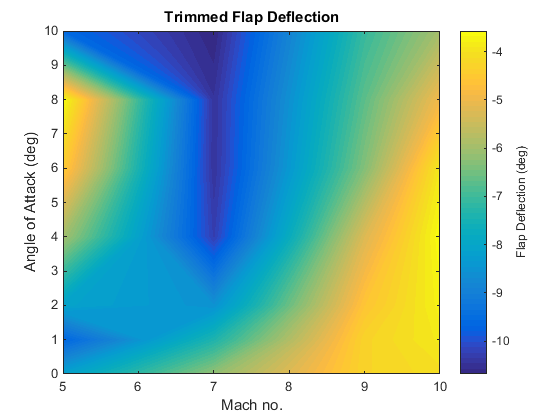
\includegraphics[width=0.99\linewidth]{figures/3_vehicle_design/FlapDeflectionENgineOn}
				\caption{Full fuel, before third stage release}
			\end{subfigure}
			\begin{subfigure}{.5\textwidth}
				\centering
				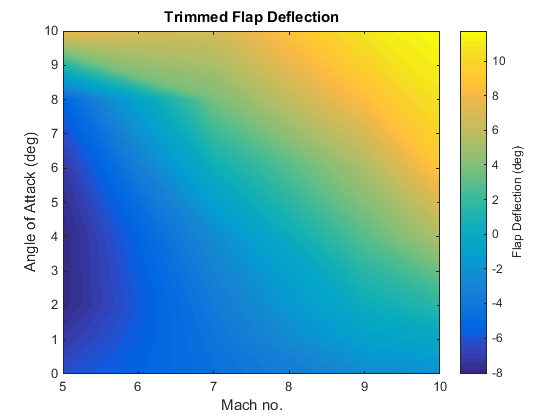
\includegraphics[width=0.99\linewidth]{figures/3_vehicle_design/FlapDeflectionENgineOn2}
				\caption{Empty of fuel, before third stage release}
				\label{fig:FlapDeflectionENgineOn2}
			\end{subfigure}
			\begin{subfigure}{.5\textwidth}
				\centering
				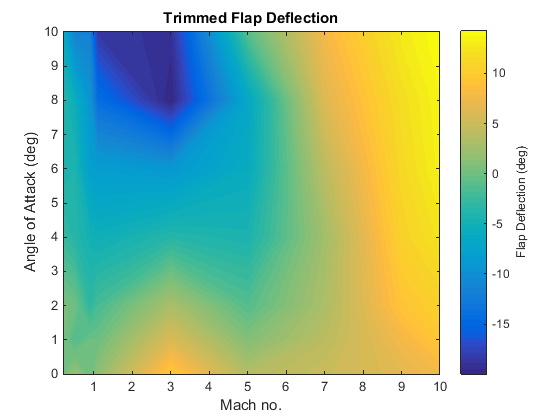
\includegraphics[width=0.99\linewidth]{figures/3_vehicle_design/FlapDeflection}
				\caption{Empty of fuel, after third stage release}
				\label{fig:FlapDeflectionEngineOff}
			\end{subfigure}
			\caption{Flap deflection required for trim of the SPARTAN. Negative up. \textit{These images will be modified when the final aerodynamics are calculated. The colourmap will be modified to have the same range across figures.}}
			\label{fig:FlapDeflection}
		\end{figure}
		
		
		
		
		
		
		\subsubsection{Database Generation}
		The trimmed aerodynamic databases of the SPARTAN are generated in full prior to trajectory simulation to improve the computational efficiency of the simulation. The aerodynamic coefficients of lift, drag and moment are tabulated, and these tables are interpolated between during simulation. 
The process for generating the aerodynamic databases is shown in Figure \ref{fig:FlowChart}. 
				\begin{figure}[ht]
					\centering
					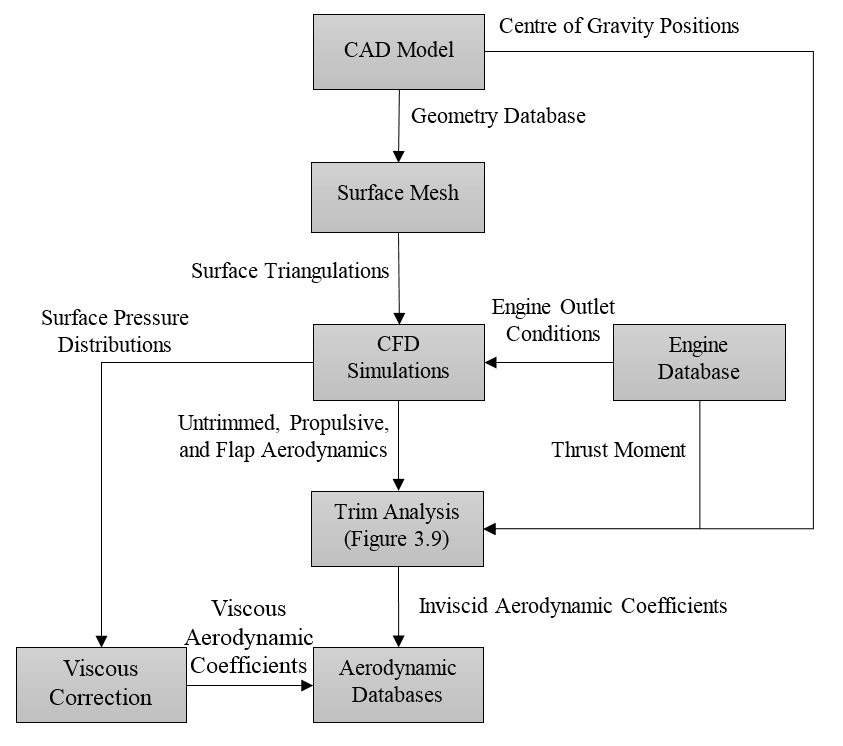
\includegraphics[width=0.7\linewidth]{figures/3_vehicle_design/FlowChart}
					\caption{Process for generating aerodynamic databases.}
					\label{fig:FlowChart}
				\end{figure}
		An initial surface triangulation of the SPARTAN is created in Pointwise, shown in Figure \ref{fig:Pointwise}. This is then imported into CART3D as a watertight surface. 
				\begin{figure}[ht]
					\centering
					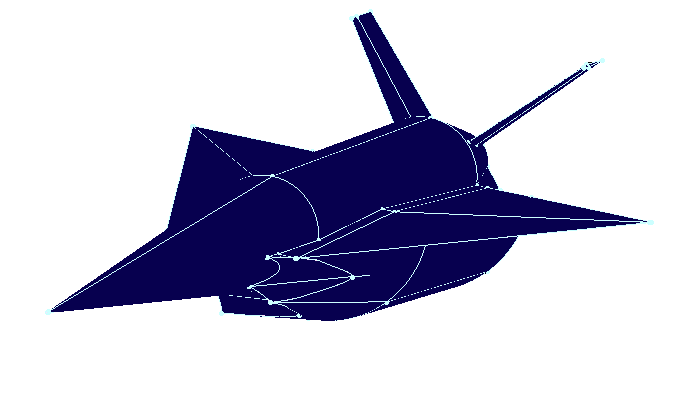
\includegraphics[width=0.6\linewidth]{figures/3_vehicle_design/Pointwise}
					\caption{Surface triangulation of the Baseline SPARTAN. \textit{This image will be recoloured.}}
					\label{fig:Pointwise}
				\end{figure}

		
		Following simulation in CART3D over the required flight conditions, the aerodynamic databases were generated. The simulation files are processed using Clic, a subprogram of CART3D used to calculate aerodynamic forces and moments, given surface pressure distributions. The solutions were processed for the necessary centre of gravity positions. At each flight conditions data point, and for each centre of gravity position, the necessary flap deflection for trim are calculated. The additional lift and drag generated by the flap are added to the untrimmed aerodynamics to create a trimmed database. 
		
		
		
		

		
		\subsubsection{Engine-On Aerodynamics}\label{sec:engine-on}
		
		The engine-on aerodynamics of the SPARTAN are used during the simulation of the acceleration phase, when the C-REST engines are operational at all times, as well as during the fly-back phase, when the engines are operational for a short time to aid the SPARTAN in returning to its initial launch site. 		
		The plumes of the SPARTAN are simulated using CART3D, using SurfBC boundary conditions which produce inflow and outflow conditions at the inlet and exit of the scramjet engines\cite{Pandya2004}. The exit conditions calculated by the CRESTM10 database, as defined in Section \ref{sec:Propulsion}, are set as the outflow conditions for the CART3D surface. The scaled engine modelled in the CRESTM10 propulsion analysis has an exit area of 0.5586m$^2$, smaller than the nozzle exit area on the SPARTAN, of 0.9719m$^2$. 
		 To accommodate for this, the outflow surfaces are scaled to the exit area of the C-Rest engines simulated by quasi 1-D analysis, to ensure that the outflow conditions match the required nozzle position. The outflow surfaces are positioned inside the nozzle on the SPARTAN model, so that the area of the outflow surface is 0.5586m$^2$. The surface triangulation of the SPARTAN with outflow surfaces is shown in Figure \ref{fig:Pointwise-EngineBC}.
				\begin{figure}[ht]
					\centering
					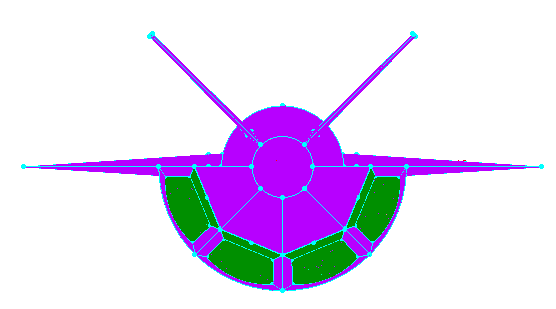
\includegraphics[width=0.7\linewidth]{figures/3_vehicle_design/Pointwise-EngineBC}
					\caption{Pointwise view of the SPARTAN showing engine outlet boundaries.}
					\label{fig:Pointwise-EngineBC}
				\end{figure}
		 CART3D performs simulations nondimensionally, and requires the outflow conditions of a boundary to be normalised. The outflow conditions of $P_e$, $rho_e$ and $M_e$ given by the CRESTM10 propulsion model are normalised to CART3D nondimensionalised variables as follows CITATIONXX;
		
		\begin{equation}
		P_e^* = P_e/(\gamma_0 P_0),
		\end{equation}
		
		\begin{equation}
		\rho_e^* = \rho_e/\rho_0,
		\end{equation}
		
		\begin{equation}
		M_e^* = \sqrt{\gamma_e/\gamma_0 (M_e \sqrt{ P_e^*/\rho_e^*})^2}.
		\end{equation}
		Where $^*$ indicates the nondimensionalised input to CART3D. This nondimensionalisation includes a correction on the Mach number to account for $\gamma_e$ variation, which is not possible to include directly in CART3D\cite{Mehta2016}. Engine-on aerodynamic calculations are performed for Mach numbers 5,7,9 and 10, and at altitudes from 20km to 40km.
		The plumes of the scramjet engines exit the nozzle of the SPARTAN, and are further expanded onto the boat tail on the rear of the SPARTAN fuselage, shown in Figure \ref{fig:EngineOn-M7AoA624km}. This expansion causes significant force on the boat tail of the SPARTAN, generating additional lift, thrust and moment forces. The trimmed aerodynamics of the SPARTAN with C-REST engines on are shown in Figure \ref{fig:EngineOnAero}.
		
		
		\begin{figure}[ht]
			\centering
			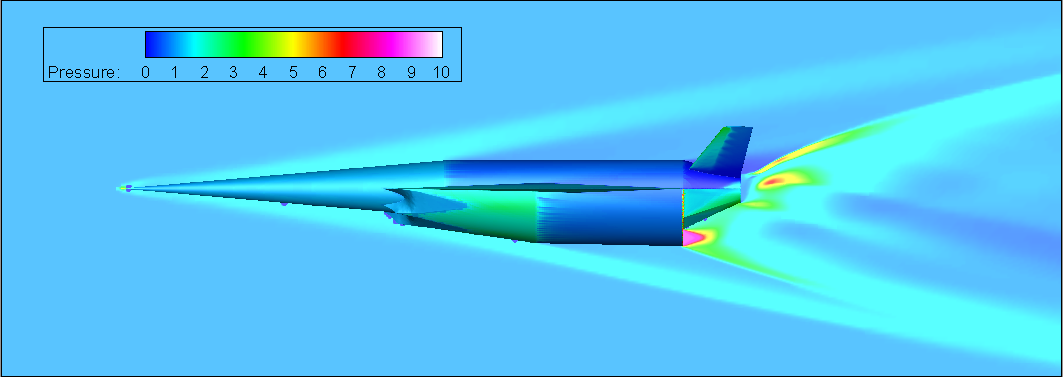
\includegraphics[width=0.9\linewidth]{figures/3_vehicle_design/EngineOn-M7AoA024km}
			\caption{Engine-on CART3D simulation at Mach 7, 6$^\circ$ angle of attack, and 24km altitude. \textit{The quality of these images will be improved.}}
			\label{fig:EngineOn-M7AoA624km}
		\end{figure}
		
		
		\begin{figure}[ht]
			\begin{subfigure}{.5\textwidth}
				\centering
				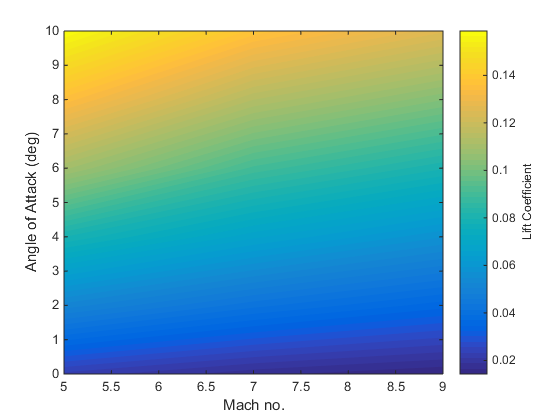
\includegraphics[width=0.99\linewidth]{figures/3_vehicle_design/Cl-EngineOn}
				\caption{Coefficient of lift.}
				\label{fig:Cl-EngineOn}
			\end{subfigure}
			\begin{subfigure}{.5\textwidth}
				\centering
				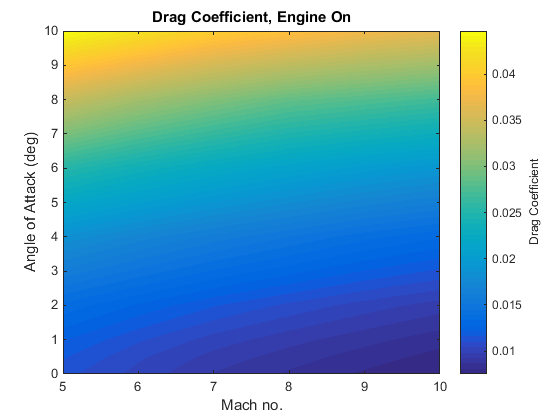
\includegraphics[width=0.99\linewidth]{figures/3_vehicle_design/Cd-EngineOn}
				\caption{Coefficient of drag.}
				\label{fig:Cd-EngineOn}
			\end{subfigure}
			\begin{subfigure}{.5\textwidth}
				\centering
				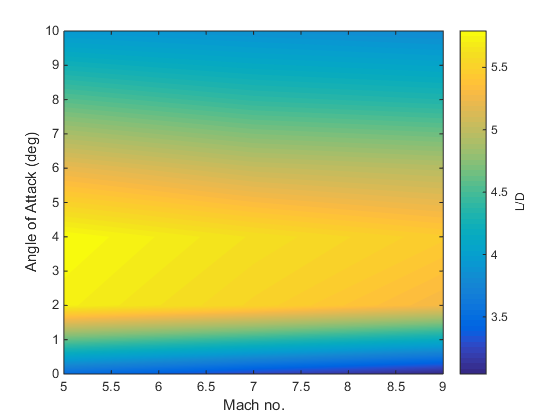
\includegraphics[width=0.99\linewidth]{figures/3_vehicle_design/LD-EngineOn}
				\caption{L/D.}
				\label{fig:LD-EngineOn}
			\end{subfigure}
			\caption{Trimmed aerodynamic coefficients with the C-REST engines powered on. Coefficients correspond to a reference area of 62.77m$^2$. }
			\label{fig:EngineOnAero}
		\end{figure}
		

\subsubsection{Engine-Off Aerodynamics}


\begin{figure}[ht]
	\centering
	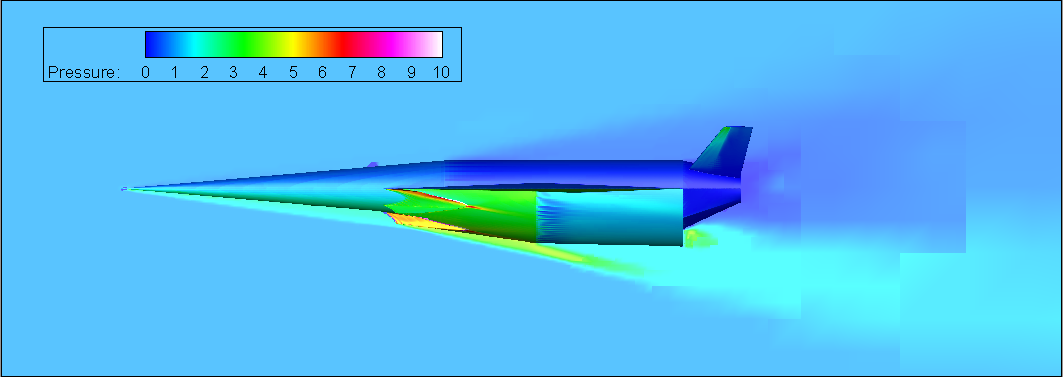
\includegraphics[width=0.9\linewidth]{figures/3_vehicle_design/M7AoA6}
	\caption{CART3D flow result for the SPARTAN, at Mach 7, 6$^\circ$ angle of attack.}
	\label{fig:M7AoA6}
\end{figure}

\begin{figure}[ht]
	\begin{subfigure}{.5\textwidth}
		\centering
		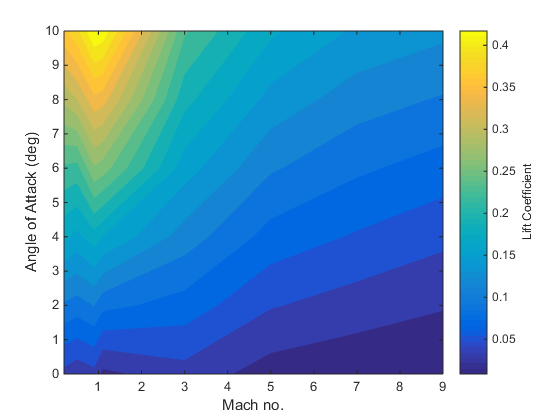
\includegraphics[width=0.99\linewidth]{figures/3_vehicle_design/Cl}
		\caption{Coefficients of lift of the SPARTAN, calculated using CART3D.}
		\label{fig:Cl}
	\end{subfigure}
	\begin{subfigure}{.5\textwidth}
		\centering
		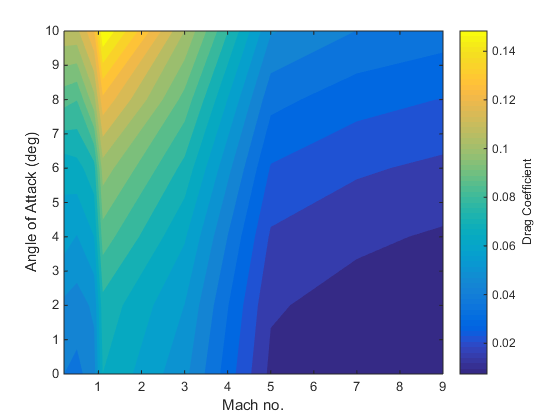
\includegraphics[width=0.99\linewidth]{figures/3_vehicle_design/Cd}
		\caption{Coefficients of drag of the SPARTAN, calculated using CART3D.}
		\label{fig:Cd}
	\end{subfigure}
	\begin{subfigure}{.5\textwidth}
		\centering
		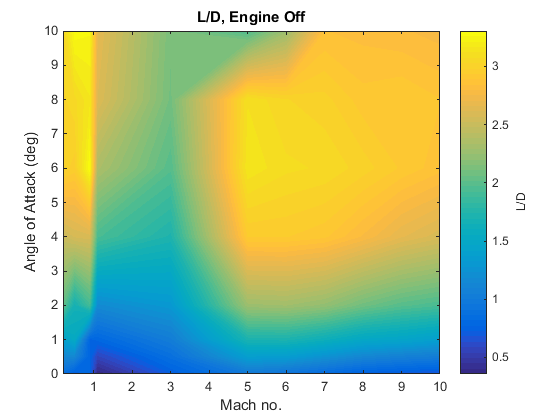
\includegraphics[width=0.99\linewidth]{figures/3_vehicle_design/LD}
		\caption{L/D of the SPARTAN.}
		\label{fig:LD}
	\end{subfigure}
	\caption{Trimmed aerodynamic Characteristics of the SPARTAN with C-REST engine powered off. Coefficients correspond to a reference area of 62.77m$^2$.}
	\label{fig:aero1}
\end{figure}

During the majority of the return flight, the scramjet engines are not operational, and the SPARTAN is gliding without power. The return phase takes the SPARTAN from third stage separation, at approximately Mach 9, to landing approach at low subsonic speeds. 
 While the engines are not powered on air flows through the flowpath without fuel injection, generating a large amount of drag. 
The aerodynamics of the SPARTAN are calculated using CART3D for Mach numbers from 0.2 to 10, and angle of attack values from 0$^\circ$ to 10$^\circ$ to cover the range of flight conditions experienced during the fly-back of the SPARTAN.  An example CART3D solution is shown for a Mach 7 engine off condition in Figure  \ref{fig:M7AoA6}. 
Figure \ref{fig:aero1} shows the engine off aerodynamic characteristics of the SPARTAN vehicle over the range of Mach numbers and angle of attack values analysed.
These results show a distinct maximum region in the L/D of the SPARTAN at high Mach numbers, within the hypersonic regime. Below Mach 5, the L/D of the SPARTAN decreases sharply. This is caused by the scramjet engines unstarting, generating significant drag. The unstarted scramjet engines are shown in Figure \ref{fig:Unstart}.

\begin{figure}[ht]
	\centering
	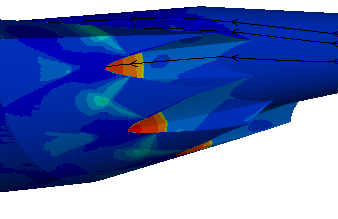
\includegraphics[width=0.7\linewidth]{figures/3_vehicle_design/Unstart}
	\caption{Unstarted scramjet engines at mach 3, 2$^\circ$ angle of attack.}
	\label{fig:Unstart}
\end{figure}


\section{First Stage Rocket}
The first stage rocket is required to deliver the second stage to near horizontal flight at Mach 5.1 flight conditions,
after which it is discarded. To achieve this, the first stage rocket is modelled as a Falcon-1e first stage scaled down
lengthwise to 9.5m, keeping the original diameter of 1.67m[CITATIONXX]. 
The Falcon-1e has been chosen due to its appropriate scale, and the proven flightworthiness of the Falcon-1. 
 The first stage is attached to the rear of the scramjet
second stage and is powered by a single LOX-kerosene Merlin 1-C engine. A connecting cowl has been modelled between the first stage rocket and the SPARTAN to improve the aerodynamic profile.  The first stage has a structural mass of
1356kg, determined by scaling of the structural mass of the Falcon-1e. The engine mass of the Merlin 1-C is kept constant during scaling at 630kg[CITATIONXX]. The mass of the
fuel in the first stage is scaled as part of the optimisation routine, as the dynamics of the vehicle, and its ability to reach a
given separation point, are very closely coupled to the available fuel mass.

The thrust and specific impulse of the Merlin 1-C are determined by interpolation between the sea level and vacuum specific impulse of the Merlin 1-C, shown in Table \ref{tab:1stStageEngine}, with pressure. Thrust scaling is determined by linear pressure scaling using nozzle exit area, $T = T_{SL} + (p_e - p_{SL})A_e$. 
 The Merlin 1-C is throttled down to a constant 85\% to allow the first stage to pitch over more easily.

\begin{table}[h]
	\centering
	\begin{tabular}{|c|c|}
		\hline  $I_{SP_{SL}}$ & 275s \\ 
		\hline  $I_{SP_{vac}}$ & 304s\\ 
		\hline  $T_{SL}$ & 555.9kN \\ 
		\hline  $A_{e}$ & $0.552m^2$ \\ 
		\hline 
	\end{tabular} 
	\caption{First Stage Engine Properties [CITATIONXX].}
	\label{tab:1stStageEngine}
\end{table}


  \subsection{Aerodynamics Including First Stage}
  
  The aerodynamics of the launch system during first stage flight are calculated in a similar manner to those of the SPARTAN without the first stage rocket, as detailed in Section \ref{sec:aero}. 
  The aerodynamics of the SPARTAN and first stage rocket are calculated using CART3D. The first stage aerodynamics are modelled between angles of attack of 0$^\circ$ to -5$^\circ$, as the first stage will be flying at negative angle of attack to induce faster pitch-over. Mach numbers from 0.2 to 5.1 (second stage separation velocity) are simulated. Figure \ref{fig:CARTcontour} shows an example CART3D simulation case, at Mach 2, -1$^\circ$ angle of attack. The coefficient of lift, drag and aerodynamic moment are tabulated for each simulation. Figure \ref{fig:FirstStageAero} shows the lift and drag coefficients of the first stage, as well as the lift-over-drag, across the simulated Mach Numbers and angles of attack. 
  Before the trajectory is simulated, the launch vehicle is trimmed using the ailerons of the SPARTAN. The simulations of the SPARTAN with flap deflections between -20$^\circ$ and 20$^\circ$ are used to calculate the deflection necessary to trim the vehicle, as described in Section \ref{sec:trim}, and the additional lift and drag generated by the ailerons is added to the aerodynamic database of the first stage launch vehicle. 
  
  
  
  \begin{figure}
  	\centering
  	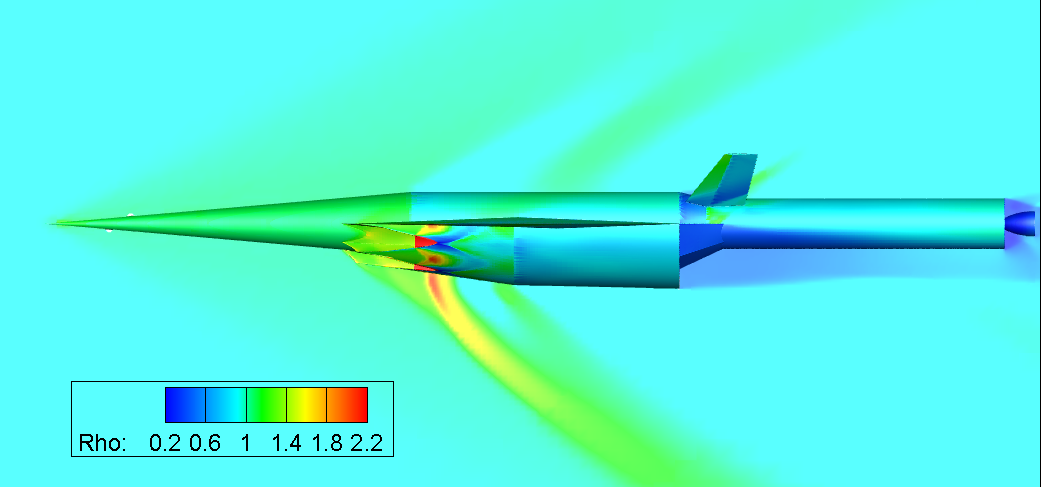
\includegraphics[width=0.7\linewidth]{figures/3_vehicle_design/CARTcontour}
  	\caption{CART3D result for the SPARTAN and first stage vehicles at Mach 2, -1$^\circ$ angle of attack.}
  	\label{fig:CARTcontour}
  \end{figure}

\begin{figure}
	\begin{subfigure}{.5\textwidth}
		\centering
		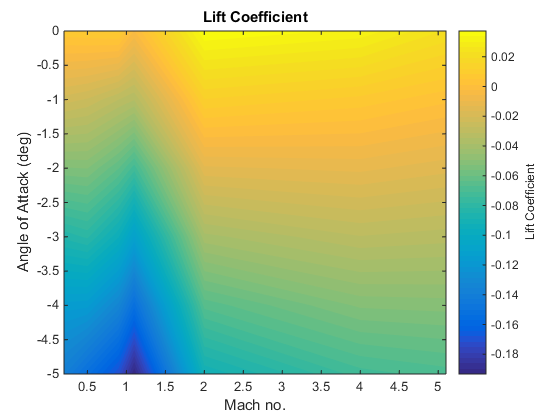
\includegraphics[width=0.99\linewidth]{figures/3_vehicle_design/FirstStageCl}
		\caption{Coefficient of lift.}
		\label{fig:Cl-FirstStage}
	\end{subfigure}
	\begin{subfigure}{.5\textwidth}
		\centering
		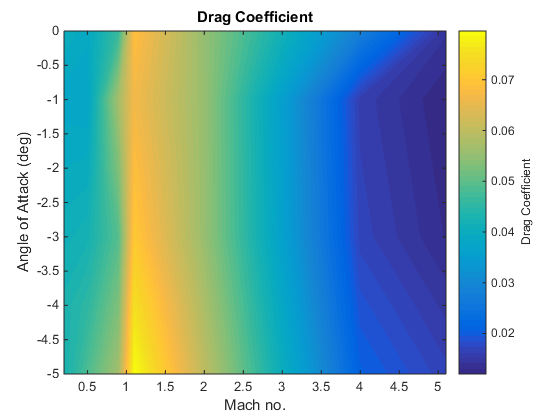
\includegraphics[width=0.99\linewidth]{figures/3_vehicle_design/FirstStageCd}
		\caption{Coefficient of drag.}
		\label{fig:Cd-FirstStage}
	\end{subfigure}
	\begin{subfigure}{.5\textwidth}
		\centering
		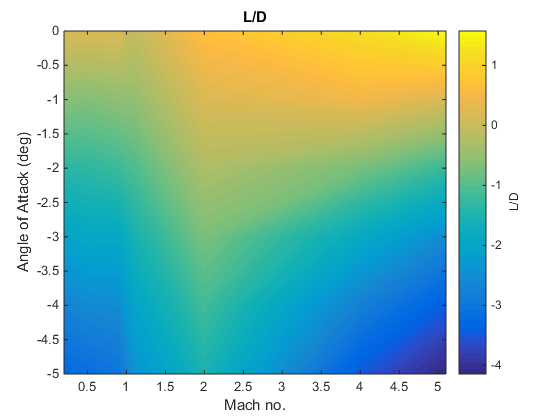
\includegraphics[width=0.99\linewidth]{figures/3_vehicle_design/FirstStageLD}
		\caption{L/D.}
		\label{fig:LD-EFirstStage}
	\end{subfigure}
	\caption{Aerodynamic characteristics of the SPARTAN including the first stage rocket.}
	\label{fig:FirstStageAero}
\end{figure}


	

	\section{Third Stage Rocket - Baseline}\label{sec:ThirdStageBaseline}
	
	\begin{figure}
\centering
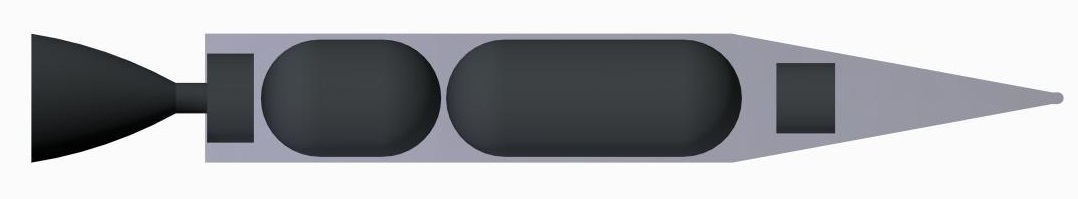
\includegraphics[width=0.7\linewidth]{figures/3_vehicle_design/3rdStage}
\caption{The third stage rocket, showing major internal features. \textit{Labels to be added.}}
\label{fig:3rdStage}
\end{figure}
	
	
	The third stage has a total length of 9m, with a 3m long nose, 4.5m long centrebody and 1.5m long engine.
	In this study the third stage rocket has been designed to accommodate a SpaceX Kestrel engine. In previous studies, the third stage has been designed to be powered by a Pratt \& Whitney RL-10-3A pump-fed engine. The Kestrel has been used over the RL-10-3A for its cost effectiveness. As a pressure-fed engine, the Kestrel trades off specific impulse for weight and cost savings when compared to the RL-10-3A. As the only expendable portion of the system; the cost of the third stage is one of the main drivers of overall system cost. Reducing the cost of the third stage allows the cost of launch to be directly reduced. 
	
	The third stage rocket is released at the end of the scramjet accelerator burn, and lifts the payload out of the atmosphere and into the desired orbit. The third stage weighs a total of 3300kg. This has been chosen as a nominal design weight, to satisfy the fuel necessary to achieve orbit with an acceptable payload, while also allowing for ample payload volume. The internal layout of the third stage rocket is shown in Figure \ref{fig:3rdStage}. The third stage has a structural mass fraction of 0.09, similar to the Falcon 1 second stage \cite{Vehicle2008}. This gives a total structural mass (without heat shield) of 285.7kg. 
	
	

	
The kestrel engine used in the third stage is modified to have 50\% increased propellant mass flow rate, giving a mass flow rate of 14.8kg/s. The nozzle exit of the Kestrel engine has been kept constant at 1.1m diameter. An increase in mass flow necessitates a corresponding increase in throat area. This increase in throat area decreases the area ratio of the nozzle. The initial area ratio is 60, measured from schematics in the Falcon-1 Users Guide. A 50\% mass flow increase corresponds to a 50\% throat area increase, which causes the area ratio to decrease to 40. This decrease in area ratio results in a 2\% loss of efficiency from the nozzle, measured from the thrust coefficient relationships shown in Figure \ref{fig:ThrustCoefficient-Arat}\cite{RPE}. The coefficient of thrust is calculated for a specific heat ratio of 1.20, as this is close to the specific heat ratio of oxygen and RP-1 of 1.24\cite{RPE}. The modified specific impulse of the engine is 310.7s.



	
	
	\begin{figure}[ht]
\centering
\includegraphics[width=0.7\linewidth]{"figures/3_vehicle_design/Thrust Coefficient - Arat"}
\caption{Variation in coefficient of thrust with area ratio \cite{RPE}.}
\label{fig:ThrustCoefficient-Arat}
\end{figure}



\subsection{Heat Shield Sizing}

The third stage rocket is separated from the SPARTAN at a high dynamic pressure, after which it spends a considerable amount of time accelerating in-atmosphere before reaching exoatmospheric conditions. The time spent within a high dynamic pressure environment creates a large amount of heat loading, which must be mitigated by heat shielding. The heat shielding must be capable of withstanding the extremely high heat and structural loading necessary to protect the third stage rocket internals and payload, as well as being lightweight, as the payload-to-orbit is extremely sensitive to the mass of the third stage, and cost effective, as increasing the cost of the third stage directly increases launch cost due to it being expendable. 


The heat shield used to protect the third stage is constructed from a tungsten nose tip, a reinforced carbon-carbon nose cone, and a phenolic cork cylinder, weighing 130.9kg in total. This heat shield is designed based on the materials and thicknesses defined in\cite{Preller2017b}. A mass breakdown is shown in Table \ref{tab:heatshield}.
Tungsten is used at the tip of the nose cone, the area of maximum heat loading. Tungsten has extremely high heat resistivity, and a very low coefficient of thermal expansion[CITATIONXX]. However, tungsten is costly and heavy, and is only used on the very tip of the nose where it is absolutely necessary. 
  Reinforced carbon-carbon is used for the conical section of the heat shield, as this is an area that will be subject to high heat and structural loading. Carbon-carbon is able to withstand high temperatures, as well as being thermal shock resistant and having a low coefficient of thermal expansion\cite{Fitzer}. Carbon-carbon is used in rocket and missile nose cones, as well as on aircraft leading edges due to its good heat resistant properties\cite{Fitzer}. However, carbon-carbon is expensive, and is used only on the conical section of the heat shield to minimise cost. For the cylindrical section of the heat shield protecting the main body of the third stage, phenolic cork is used. Phenolic cork is a composite of ground cork and phenolic binders which is light and relatively cheap, with good heat resistivity. Phenolic cork has lower tensile strength and heat resistivity than carbon-carbon\cite{Composites,Fitzer}, but is cheaper and lighter, making it appropriate for use on section of the heat shield which experiences lower heating and structural loads. 

		\begin{table}[h]
			\centering
\begin{tabular}{|c|c|c|c|}
	\hline  Part & Density & Geometry & mass \\ 
	\hline  Tungsten Nose & $\rho_{Tungsten} = 19250$  kg/m$^3$ & 50mm diameter cylinder, spherical tip & 12.6kg \\ 
		\hline C-C Cone & $\rho_{CC} = 1800$  kg/m$^3$ & 10mm thick, conical & 93.4kg \\ 
			\hline Phenolic Cork Cylinder & $\rho_{Phenolic Cork} = 320$  kg/m$^3$ & 5mm thick, cylindrical & 24.9kg \\ 
	\hline 
\end{tabular} 
\caption{Third stage heat shield breakdown.}
\label{tab:heatshield}
\end{table}
		
		\subsection{Fuel Tank Sizing}
		The internal design of the third stage is allowed to be slightly variable as the trajectory is optimised. The third stage mass is fixed at 3300kg, and the calculated payload-to-orbit varies by exchanging leftover fuel mass for effective payload mass. To calculate the dynamics of the third stage, the fuel tanks have been approximately sized, assuming 160kg of payload-to-orbit. Realistically the exchange between fuel and payload mass would cause the fuel tanks to be resized slightly. For the purposes of this study the fuel tanks are assumed to be of constant size for simplicity. Currently this is a reasonable assumption as the internals of the rocket are very simplified. The structural mass is held constant at 9\%. The third stage carries a total propellant mass of 2736.7kg. Table \ref{tab:Fuel} breaks shows the component break-down of the LOX oxidiser and RP1 fuel.  
		
		\begin{table}[h]
			\centering
\begin{tabular}{|c|c|c|}
	\hline  & \textbf{LOX} & \textbf{RP1} \\ 
	\hline Ratio & 2.56 & 1 \\ 
	\hline Density & 1141kg/m3 & 813kg/m3 \cite{Magee}\\ 
	\hline Volume & 1.7248m3 & 0.9455m3 \\ 
	\hline Mass & 1968.0 kg & 768.7 kg \\ 
	\hline 
\end{tabular} 
\caption{Third stage fuel distribution.}
\label{tab:Fuel}
		\end{table}

		
		

		\subsection{The Aerodynamics of the Third Stage Rocket}
		
		The third stage aerodynamics have been calculated using Missile DATCOM [REFXX], a preliminary design tool for estimating the aerodynamic characteristics of missile and rocket vehicles. Missile DATCOM utilises empirical methods, along with various estimation techniques, to compute the aerodynamics of missile-like vehicles across the subsonic, supersonic and hypersonic regimes. The aerodynamics of the third stage rocket are shown in Figure \ref{fig:ThirdStageAero}. The code used to compute the aerodynamics of the third stage rocket is detailed in Appendix XX.  
		
		
		\begin{figure}
			\begin{subfigure}{.5\textwidth}
				\centering
				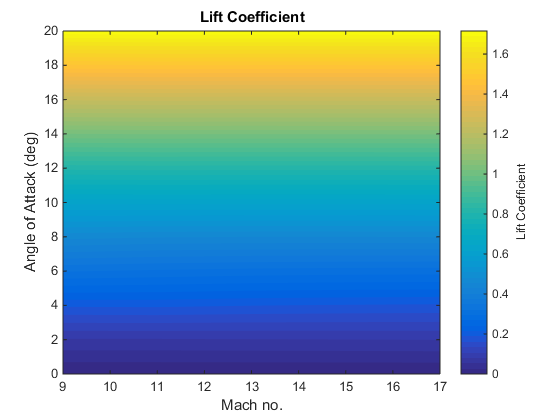
\includegraphics[width=0.99\linewidth]{figures/3_vehicle_design/ThirdStageCl}
				\caption{Coefficient of lift.}
				\label{fig:Cl-ThirdStage}
			\end{subfigure}
			\begin{subfigure}{.5\textwidth}
				\centering
				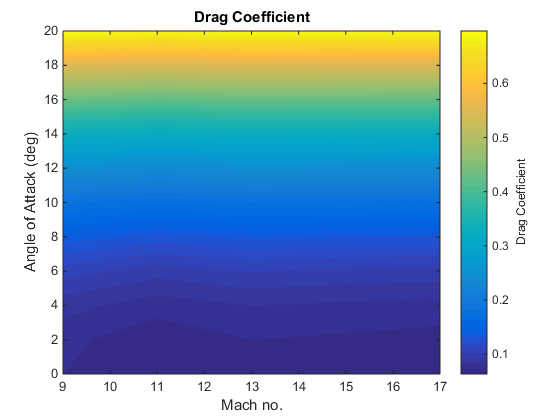
\includegraphics[width=0.99\linewidth]{figures/3_vehicle_design/ThirdStageCd}
				\caption{Coefficient of drag.}
				\label{fig:Cd-ThirdStage}
			\end{subfigure}
			\begin{subfigure}{.5\textwidth}
				\centering
				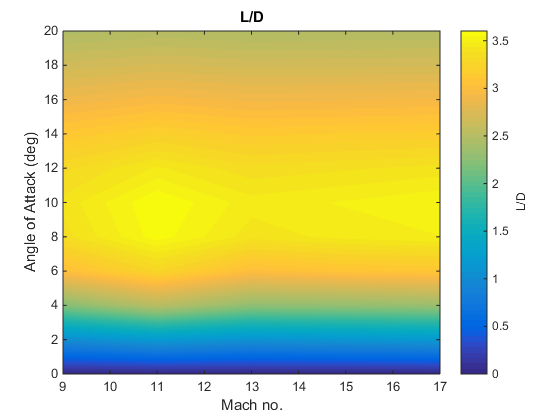
\includegraphics[width=0.99\linewidth]{figures/3_vehicle_design/ThirdStageLD}
				\caption{L/D.}
				\label{fig:LD-ThirdStage}
			\end{subfigure}
			\caption{Aerodynamic characteristics of the baseline third stage rocket, for a reference area of 0.95m$^2$.}
			\label{fig:ThirdStageAero}
		\end{figure}
		
		
		
		\subsubsection{Thrust Vectoring}
		
		The third stage rocket is controlled via thrust vectoring. The centre of pressure is calculated using missile DATCOM. The thrust vector is set so that the moment generated by the engine matches the lift force acting at the centre of pressure, shown in Figure \ref{fig:ThrustVec}. The maximum thrust vector limit has been set to 8$^\circ$. As no data on the maximum thrust vectoring capabilities of the kestrel engine was able to be found, this was set to the maximum gimbal range of the Aestus pressure-fed engine and OMS, similar pressure fed engines CITATIONXX.
		
			The centre of gravity is determined using CREO, and is at XXm from the nose. It is assumed that the mass of the structure of the rocket (excluding fuel tanks, heat shielding, engine and payload) is distributed homogeneously for simplicity.
		The third stage rocket is statically unstable. Flying this rocket at an angle of attack will require an advanced automatic controller, as the only control available is produced by thrust vectoring. This study assumes that the third stage rocket is able to be controlled over any required trajectory, as long as the thrust vector limits of the vehicle are not exceeded. 
		
		
\begin{figure}
\centering
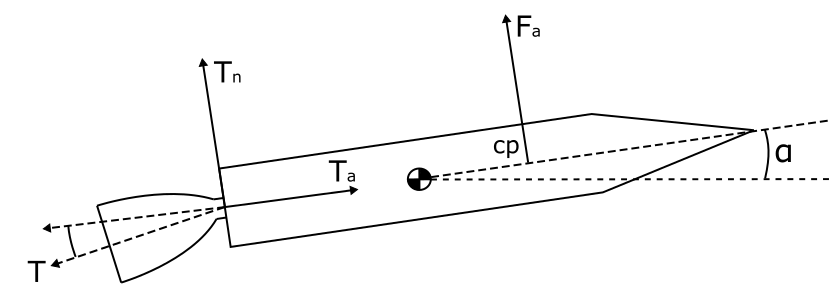
\includegraphics[width=0.6\linewidth]{figures/3_vehicle_design/ThrustVec}
\caption{Thrust vector force balance.}
\label{fig:ThrustVec}
\end{figure}
		

		